\documentclass[10pt]{article}
\usepackage{amsmath} % assumes amsmath package installed
\usepackage{amsfonts,mathrsfs}
\usepackage{amssymb}
\usepackage{color}
\usepackage{graphicx}
\usepackage{epsfig}
\usepackage{subfigure}
\usepackage{enumerate}
\usepackage{algorithm,algorithmicx}
\usepackage{algpseudocode}

%\usepackage[]{algorithm2e}

\def\bbbr{{\rm I\!R}}
%\input{macros.tex}
%\input{slide_macros.tex}

\newtheorem{definitiox	n}{Definition}{\it}{}
\newtheorem{example}{Example}{\it}{}
\newtheorem{corollary}{Corollary}{\it}{}
\newtheorem{proposition}{Proposition}{\it}{}
\newtheorem{lemma}{Lemma}{\it}{}
\newtheorem{theorem}{Theorem}{\it}{}
\newtheorem{remark}{Remark}{\it}{}
\newtheorem{assumption}{Assumption}{\it}{}
\newenvironment{proof}[1][Proof]{\noindent\textbf{#1.} }{\ \rule{0.5em}{0.5em}}
%\newcommand{\proof}{\vspace{1mm}\noindent{\it Proof.}\quad}
%\def\qed{\quad{$\square$}} 

\textwidth=6.3in
\textheight 9in 
\setlength{\topmargin}{-0.5in}
\setlength{\oddsidemargin}{0.1in} 
\setlength{\evensidemargin}{0.1in}
%%%%%%%%%%%%%%%%%%%%%%%%%%%%%%%%%%
\def\an#1{{{\bf \color{blue}#1}}}
\def\o{\omega}
\def\vmean{v^{\rm mean}}
\def\vmax{v^{\rm max}}	
\def\e{\epsilon}
\newcommand{\todo}[1]{\vspace{5 mm}\par \noindent \marginpar{\textsc{ToDo}}
\framebox{\begin{minipage}[c]{0.9 \textwidth} \tt #1
\end{minipage}}\vspace{5 mm}\par}

% Boldsymbols, mathcal, mathbb
\newcommand{\bs}{\boldsymbol}
\newcommand{\mc}{\mathcal}
\newcommand{\bb}{\mathbb}
\newcommand{\R}{\bb R}

%norm
\newcommand{\norm}[1]{\left\|#1\right\|}

% Operators and notations
\newcommand{\dom}{\operatorname{dom}}
\newcommand{\iP}{\mathcal{P}}
\newcommand{\B}{\mathcal{C}}
\newcommand{\red}{\textcolor{red}}
\newcommand{\blue}{\textcolor{blue}}
\newcommand{\argmin}{\operatorname{argmin}}
\newcommand{\mini}{\operatorname{minimize}}
\newcommand{\Proj}{\mathrm{Proj}}
\newcommand{\fix}{\mathrm{fix}}
\newcommand{\proj}{\mathrm{proj}}
\newcommand{\prox}{\mathrm{prox}}
\newcommand{\Id}{\mathrm{Id}}
\newcommand{\Res}{\operatorname{J}}
\newcommand{\diag}{\operatorname{diag}}
\newcommand{\blkdiag}{\operatorname{blkdiag}}
\newcommand{\col}{\operatorname{col}}
\newcommand{\zer}{\operatorname{zer}}
\newcommand{\nulls}{\operatorname{Null}}
\newcommand{\range}{\operatorname{Range}}
\newcommand{\dist}{\mathrm{dist}}
\newcommand{\nc}{\mathrm{N}}
\newcommand{\0}{\mathbf{0}}
\newcommand{\1}{\mathbf{1}}
\newcommand{\half}{^1\hspace*{-.1em}/_2}

%Roman numbers
\newcommand{\rmnum}[1]{\romannumeral #1}
\newcommand{\Rmnum}[1]{\expandafter\@slowromancap\romannumeral #1@}


%%%%%%%%%%%%%%%%%%%%%%%%%%%%%%%%%%%%%%%

\title{Decentralized Algorithms for Generalized Nash Equilibrium Seeking in Peer-to-peer Electricity Markets}
\author{Giuseppe Belgioioso}
\begin{document}
\maketitle

%%%%%%%%%%%%%%%%%%%%%%%%%%%%%%%%%%%%%
\section{Problem statement}
Consider the same problem statement in \texttt{problem\_setup\_v7.tex}.

%%%%%%%%%%%%%%%%%%%%%%%%%%%%%%%%%%%%%%%%%%%%%%%%%%%%%%

\section{Algorithms}
\subsection{Semi-decentralized}

The algorithm presented in this section corresponds to \cite[Alg. 6B]{belgioioso2020semi} applied on  \texttt{problem\_setup\_v6.tex}.

Consider the following choices for the step-sizes in Algorithm 1.
\smallskip

\begin{assumption}[Step-size]\label{ass:SSS}
Set the step sizes of prosumers and DSO as follows:
\begin{enumerate}[(i)]
\item $\forall i \in \mc N$: set $A_i = \diag( \alpha_{i}^{\text{pi}}, \alpha_{i}^{\text{st}} , \alpha_{i}^{\text{mg}} , \{ \alpha_{(i,j)}^{\text{tr}} \}_{j \in \mc N_i} ) \otimes I_H$, with $\alpha_{i}^{\text{pi}}, \alpha_{i}^{\text{st}} > 1$, $ \alpha_{i}^{\text{mg}} > 3 + N \max_{h\in \mc H} d_h^{\text{mg}} $, \red{$\alpha_{(i,j)}^{\text{tr}} > 2$, $\forall j \in \mc N_i$}, $\beta^{\text{tr}}_{(i,j)} = \beta^{\text{tr}}_{ (j,i)} < \frac{1}{2}$, $\forall j \in \mc N_i$. 

\item Set $A_{N+1}:=\diag\left(
\left\{
\alpha_y^{\theta},\alpha^{\text v}_y, \alpha_y^{\text{tg}},
\{ 
\alpha^\text{p}_{(y,z)}, \alpha^{\text{q}}_{(y,z)} 
\}_{z \in \mc B_y}
\right\}_{y \in \mc B}
\right) \otimes I_H
$, with $\alpha_y^{\theta},\alpha^{\text v}_y > 0$, $\alpha_y^{\text{tg}} > 2$, $\alpha^{\text{p}}_{(y,z)} > 1$ and $ \alpha^{\text{q}}_{(y,z)} > 0 $, $\forall z \in \mc B_y$, $ \forall y \in \mc B$.
Set $\gamma^{\text{mg}} < \frac{1}{N}$, $\beta^{\text{tg}} < (|\mc N| + |\mc B|)^{-1}$ and $\beta_y^{\text{pb}} < (1+|\mc N_y|+|\mc B_y|)^{-1}$, for all $y \in \mc B$.
{\hfill $\square$}
\end{enumerate}


\end{assumption}




\newpage
%%%%%%%%

\algblockdefx[DSO]{DSO}{EndDSO}
[1][<default value>]{\textbf{DSO update}}
[2][<default value>]{\textbf{end}}

\algblockdefx[Primal]{Primal}{EndPrimal}
[1][<default value>]{\textbf{primal update}}
[2][<default value>]{\textbf{end}}

\algblockdefx[Dual]{Dual}{EndDual}
[1][<default value>]{\textbf{dual update}}
[2][<default value>]{\textbf{end}}

\algblockdefx[Comm]{Comm}{EndComm}
[1][<default value>]{\textbf{communication}}
[2][<default value>]{\textbf{end}}

\algblockdefx[Agg]{Agg}{EndAgg}
[1][<default value>]{\textbf{aggregation update}}
[2][<default value>]{\textbf{end}}

\algblockdefx[IUC]{IUC}{EndIUC}
[1][<default value>]{\textbf{Iterate until convergence}}
[2][<default value>]{\textbf{end}}
%%%%%%%%%%

\begin{algorithm}[H]
\caption{Semi-decentralized GWE seeking for P2P Energy Markets}
\begin{algorithmic}[1]
	%
%\Procedure{Initialization prosumers}{}
%\ForAll{prosumer $ i \in \mc N$}
%\State  Set the initial conditions: $u_i(0) \in \mc U_i$, $\mu^{\text{tr}}_{(i,j)}(0) = \0$, $\forall j \in \mc N_i$.
%\State  Set the step sizes as in Assumption \ref{ass:SSS}(i).
%\EndFor
%\EndProcedure
%\Procedure{Initialization DSO}{}
%\State  Set the initial conditions: $u_{N+1}(0) \in \mc U_{N+1}$, $\lambda^{\text{mg}}=\0$, $\mu^{\text{tg}} = \0$, $\mu_y^{\text{pb}}(0) = \0$, $\forall y \in \mc B$.
%\State Set the step sizes as in Assumption \ref{ass:SSS}(ii).
%\EndProcedure
\medskip
\IUC{ }


\ForAll{prosumer $ i \in \mc N$}
\Primal{ }
\Comment{power generated, stored, from the grid, traded}

\smallskip
\State 
$a_i(k) = 
	\col \big(-\mu_y^{\text{pb}}(k),-\mu_y^{\text{pb}}(k),
	{
	%\left(
	\left[
	\begin{smallmatrix}
	I_H\\
	- I_H 
	\end{smallmatrix}
	\right] 
	%\otimes I_H
%\right)	
	}^\top \lambda^{\text{mg}}(k) + \mu^{\text{tg}}(k),
	%
	\left\{ {\mu^{\text{tr}}_{(i,j)}(k)}\right\}_{j \in \mc N_i}   \big)$
\Comment{aux. vector}

\State
$u_i(k+1)   =
\left\{
\begin{array}{r l}
	\underset{\xi \in \R^{n_i}}{\argmin} & 
	J_{i} \big( \xi, \sigma(k) \big) 
	+ {a_i(k)}^\top \xi + \frac{1}{2}
	\left\| \xi - u_i(k) 
	\textstyle
	  \right\|^2_{A_i} \\
	\text{s.t. } & \xi \in \mc U_i
\end{array} 
	\right.	$
\Comment{quadratic progr.}	
\EndPrimal

\Comm{ }
\Comment{to DSO and trading partners}
\State $b_i(k+1)= p^{\text{d}}_i-p^{\text{di}}_i(k+1)- p^{\text{st}}_i(k+1)$
\Comment{local load unbalance of prosumer $i$}
\State
$
p^{\textrm{mg}}_{i}(k+1), b_i(k+1)  \longrightarrow  \text{DSO,}
$
\Comment{forward to DSO}
     \ForAll{prosumer $ j \in \mc N_i$}
     
\State
 $p^{\text{tr}}_{(i,j)}(k+1)
	\longrightarrow \text{prosumer }j$
	\Comment{forward local trade to prosumer $j$}
	\EndFor
\EndComm


\Dual{ }
\Comment{reciprocity constraints}
\ForAll{$ j \in \mc N_i$}
\State
$c^{\text{tr}}_{(i,j)}(k+1)  =  p^{\textrm{tr}}_{(i,j)} (k+1) + p^{\textrm{tr}}_{(j,i)}x(k+1)$
\Comment{aux. vector}
\State
$\mu_{(i,j)}(k+1) = \mu_{(i,j)}(k) + \beta_{ij}^{\text{tr}} \left( 
	2  c^{\text{tr}}_{(i,j)}(k+1) - c^{\text{tr}}_{(i,j)}(k)
	\right)$
	\Comment{reflected dual ascent}
\EndFor

\EndDual

\EndFor

%%%%%%%%%%%%%%%%%%%%%%
%\Statex
\DSO{ }

\Primal{}
\Comment{physical variables}
\State
$a_{N+1}(k+1) = \col \left( 
	\left\{
	\0,\0,-\mu^{\text{tg}}(k) - \mu_y^{\text{pb}}(k), 
	\{ -\mu_y^{\text{pb}}(k), \0 \}_{z \in \mc B_y}
	\right\}_{y \in \mc B}
	\right)$
\Comment{aux. vector}

\State 	$u_{N+1}(k+1) = \proj_{\mc U_{N+1}}  \left( u_{N+1}(k) - A_{N+1} a_{N+1}(k) \right)$
\Comment{ solved via Algorithm 2 }
\EndPrimal

%---------------------------Aggregation
\Agg{}
\State
$ \sigma^{\text{mg}}(k+1) = \sum_{i \in \mc N} p_i^{\text{mg}}(k+1) $
\Comment{aggregate grid-to-prosumers power }
\State
$\sigma^{\text{tg}}(k+1) = \sum_{y \in \mc B} p_y^{\text{tg}}(k+1)$
\Comment{aggregate grid-to-buses power }
\EndAgg

%---------------------------Dual Update
\Dual{}
\State
$b_{N+1}(k+1	) = 
	\left[
	\begin{smallmatrix}
	1\\
	- 1 
	\end{smallmatrix}
	\right] \otimes (2 \sigma^{\text{mg}}(k+1)- \sigma^{\text{mg}}(k)) 
	-
	\left[
	\begin{smallmatrix}
	\overline{p}^{\mathrm{mg}}\1_{H} \\
	-     \underline{p}^{\mathrm{mg}} \1_{H}
	\end{smallmatrix} 
	\right]  $
	\Comment{aux. vector}
	\State
$\lambda^{\text{mg}}(k+1) = \textstyle
	\proj_{\R^{2 H}_{\geq 0}}\left( 
	\lambda^{\text{mg}}(k) + \gamma^{\text{mg}} b_{N+1}(k+1)
	 \right)$
		\Comment{grid constraints}

\ForAll{buses $ y \in \mc B$}

\State
$c^{\text{pb}}_y(k+1)   = p_y^{\text{pd}} + \sum_{i \in \mc N_y} b_i(k+1)- p^{\text{tg}}_y(k+1) - \sum_{z \in \mc B_y} p^\ell_{(y,z)} (k+1)$
\Comment{aux. vector}

\State
$\mu_y^{\text{pb}}(k+1) = \mu_y^{\text{pb}}(k) + \beta^{\text{pb}}_y (2 c^{\text{pb}}_y(k+1)- c^{\text{pb}}_y(k))$
\Comment{local power balance of bus $y$}
\EndFor

\State
$c^{\text{tg}}(k+1) = \sigma^{\text{mg}}
	(k+1)- \sigma^{\text{tg}}(k+1)$
\Comment{aux. vector}

\State
$\mu^{\text{tg}}(k+1) = \mu^{\text{tg}}(k) + \beta^{\text{tg}} (2c^{\text{tg}}(k+1)-c^{\text{tg}}(k))$
\Comment{grid-to-buses constraints}
\EndDual	

\Comm{ }
\Comment{broadcast}
\State
$ \{ \sigma(k+1), \, \lambda^{\text{mg}}(k+1), \mu^{\text{tg}}(k+1) \} 
	\longrightarrow  \mc N$
\Comment{to all prosumers}
\ForAll{buses $ y \in \mc B$}
\State
$\mu^{\text{pb}}_y(k+1)\longrightarrow \mc N_y$
\Comment{to all prosumers on bus $y$}
\EndFor

\EndComm

\EndDSO	

\EndIUC	

\end{algorithmic}
\end{algorithm}

\begin{figure}
\centering
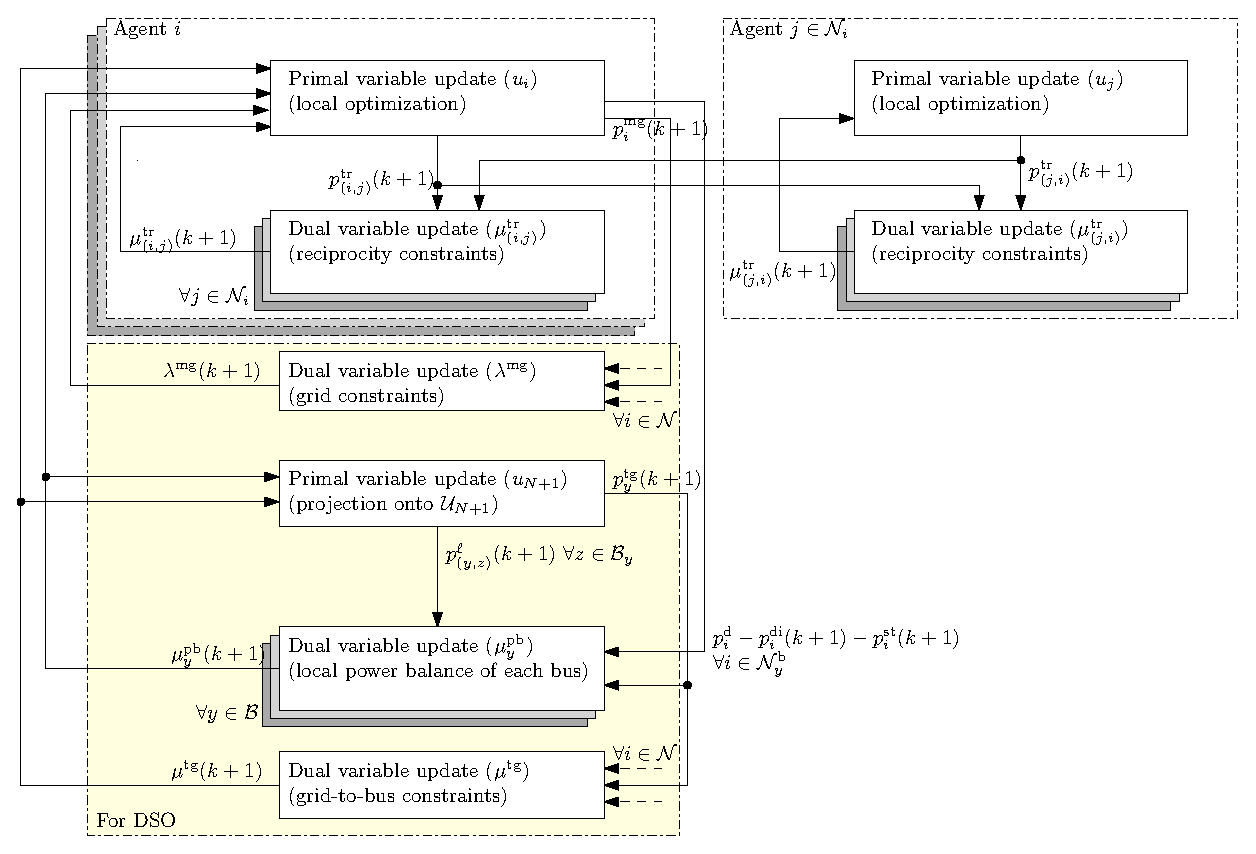
\includegraphics[scale=0.8]{Algorithm1_v2}
\caption{Flowchart of the iterations in Algorithm 1 for agent $i \in \mc N$ and DSO. It also shows the flow of information between agent $i$ and DSO as well as between agent $i$ and its trading partner $j$.}
\end{figure}

%%%%%%%%%%%%%%%%%%%%%%%%%%%%%%%%%%%%%%%%%%%

\subsection{Projection onto $\mc U_{N+1}$}
Next, we propose an iterative method to solve line 24 in Algorithm 1, namely, to compute the projection onto $\mathcal{U}_{N+1}$. First, let us define the sets $C_1 := (17)\cap(18)\cap(19)\cap(20) $ and $C_2 = (15)\cap(16)$ and recall that the decision vector of the DSO reads as $u_{N+1}=\col\left(\{\theta_y, v_y, p_y^{\mathrm{tg}},\{p_{(y,z)}^{\ell},q_{(y,z)}^{\ell}\}_{z \in \mc B_y} \}_{y\in\mc B} \right)$. The projection onto $C_1$ can be characterize in closed-form as follows:
\begin{align*}
\proj_{C_1}(u_{N+1})=
\col\left(\{\theta_y^+, v_y^+, {p_y^{\mathrm{tg}}}^+,\{ {p_{(y,z)}^{\ell}}^+, {q_{(y,z)}^{\ell}}^+ \}_{z \in \mc B_y} \}_{y\in\mc B} \right),
\end{align*}
where, for all $y \in \mc B$,
\begin{align*}
\theta_y^+ &=
\begin{cases}
\underline{\theta}_y, & \text{if } \theta_y < \underline{\theta}_y\\
\overline{\theta}_y, & \text{if } \theta_y > \overline{\theta}_y\\
\theta_y, & \text{otherwise } \
\end{cases}, &  \\
%
v_y^+ &= 
\begin{cases}
\underline{v}_y, & \text{if } v_y < \underline{v}_y\\
\overline{v}_y, & \text{if } v_y > \overline{v}_y\\
v_y, & \text{otherwise } \
\end{cases}
 & \\
%
{p_y^{\text{tg}}}^+ &= 
\begin{cases}
p_y^{\text{tg}}, & \text{if } y \in \mc B^{\text{mg}}\\
0, & \text{otherwise} 
\end{cases}
\\
%
{(p^\ell_{(y,z),h})}^+ & = \frac{\overline{s}_{(y,z)}}{
\max \left\{ \|\col(p^\ell_{(y,z),h)} , q^\ell_{(y,z),h)} \|, \overline{s}_{(y,z)} \right\}
} p^\ell_{(y,z),h},& \quad \forall z \in \mc B_y, \forall h \in \mc H \\
{(q^\ell_{(y,z),h})}^+ & = \frac{\overline{s}_{(y,z)}}{
\max \left\{ \|\col(p^\ell_{(y,z),h)} , q^\ell_{(y,z),h)} \|, \overline{s}_{(y,z)} \right\}
} q^\ell_{(y,z),h} , & \quad \forall z \in \mc B_y, \forall h \in \mc H
\end{align*}
The projection onto $C_2$ can be computed by solving a quadratic programming (e.g. via lsqlin, quadprog, osqp, etc...) with appropriate matrices.

\begin{algorithm}[]
\caption{Douglas--Rachford splitting to compute the projection of $x$ onto $\mathcal{U}_{N+1} = C_1 \cap C_2$}
\begin{algorithmic}[1]

\smallskip
\IUC{ }

\smallskip
\State
$z(k) = \proj_{C_1}(\frac{1}{2} \xi(k) + \frac{1}{2}x)$ 


\smallskip
\State
$\xi(k+1) = \xi(k) + \lambda \left( \proj_{C_2}    (2z(k)-\xi(k)) - z(k)
\right), \quad \text{ with } \lambda \in (0,2)
$
\EndIUC

\end{algorithmic}
\end{algorithm}

\newpage

%%%%%%%%%%%%%%%%%%%%%%%%%%%%%%%%%%%%%%%%%%%%%%%%
\newpage
\subsection{Fully-distributed}

The algorithm presented in this section is a variation of \cite[Alg. 3]{belgioioso2019distributed} for the setup considered in the ECC 2020 paper.

Consider the following mixing matrix.
\begin{assumption} \label{ass:DSMM}
For all $k \in \bb N$, the matrix $W=[w_{i,j}] $ satisfies the following conditions:
\begin{enumerate}[(i)]
\item (Edge utilization) Let $i,j \in \mc I$, $i \neq j$. If $(i,j) \in \mc E_k$, $w_{i,j} \geq \epsilon$, for some $\epsilon > 0$; $w_{i,j} = 0$ otherwise;
\item (Positive diagonal) For all $i \in \mc I$, $w_{i,i} > \epsilon$;
\item (Double-stochasticity) $W \1 = \1$, $\1^\top W = \1^\top$.
{\hfill $\square$}
\end{enumerate}
\end{assumption}

\smallskip
Assumption \ref{ass:DSMM} is strong but typical for multiagent coordination and optimization \cite{margellos2018distributed}. For an undirected graph it can be fulfilled, for example, by using Metropolis weights:
\begin{equation} \label{eq:Metropolis}
w_{i,j}=
\begin{cases}
(\max\{|\mc N_i|, |\mc N_j| \})^{-1} & \text{if } (i,j) \in \mc E,\\
0 & \text{if } (i,j) \not\in \mc E, %\, i \neq j,
\\
1- \sum_{\ell \in \mc N_i} w_{i,\ell} & \text{if } i=j.
\end{cases}
\end{equation}

\medskip

Consider the following choices for the step-sizes in Algorithm 2.

\begin{assumption}[Step size selection]\label{ass:SS-choiceFD}
For all $i \in \mc N$, set $A_i = \blkdiag(  A_{i,1},\ldots, A_{i,H})$, where $A_{i,h} = \diag \left(
\alpha_{i,h}^{\mathrm{dg}},  \; \alpha_{i,h}^{\mathrm{st}},\;  \alpha_{i,h}^{\mathrm{mg}}, \; \{ \alpha_{(i,j),h}^{\mathrm{tr}} \}_{j\in\mathcal{N}_i} \right)$, for all $ h \in \mc H$, with $\alpha_{i,h}^{\mathrm{dg}}, \; \alpha_{i,h}^{\mathrm{st}}>0$, $\alpha_{i,h}^{\text{mg}} > q_{h}^{\text{mg}} + 1$ and $\alpha_{(i,j),h}^{\mathrm{tr}} > |\mc N_i|$, for all $ j \in \mc N_i$; $\beta_{(i,j)} = \beta < \frac{1}{2}$ for all $j \in \mc N_i $; $\gamma < 1.$

{\hfill $\square$}
\end{assumption}

\begin{assumption}[Kransol'skii--Mann step] \label{ass:van-ss} The sequence $( \delta(k) )_{k \in \bb N}$ satisfies the following conditions:
\begin{enumerate}[(i)]
\item (non-increasing) $0 \le \delta(k)^{k+1} \le \delta(k) \le 1$, for all $k \ge 0$;
\item (non-summable) $\sum_{k=0}^\infty \delta(k) = \infty$;
\item (square-summable) $\sum_{k=0}^\infty {\delta(k)}^2 < \infty$.
{\hfill $\square$}
\end{enumerate}
\end{assumption}

\begin{remark}[Vanishing KM steps seem not necessary in practice]
For the numerical studies, we can use $\delta(k)=1$, for all $k \in \bb N$.
\end{remark}



\begin{algorithm}[H]

	\caption{Fully-Distributed GWE seeking for P2P Energy Markets}
	
	\medskip
	\noindent
	%
	\textbf{Initialization}:
	For all $ i \in \mc N$, set locally:
	\begin{enumerate}[(a)]
		\item Initial conditions: $u_i(-1), u_i(0), \tilde u_i(-1) \in \mc U_i$, $\mu_{(i,j)}(0) = \0$ for all $ j \in \mc N_i$, $\lambda_i(0) \in \R^{2H}_{\geq 0}$, $\sigma_i(0)=x_i(0)$, $z_i(0) = \lambda_i(0)$, $y_i(0) = 2\tilde u_i(-1)- u_i(-1) -  \frac{1}{N} \left[
	\begin{smallmatrix}
	\overline{p}^{\mathrm{mg}}\1_{H} \\
	-     \underline{p}^{\mathrm{mg}}N \1_{H}
	\end{smallmatrix} 
	\right]  		
		$.
		
		\item Step-sizes:
$A_i$, $\{\beta_{ij}\}_{j \in \mc N_i}$ and $\gamma_i$ as in Assumption \ref{ass:SS-choiceFD}; $\{ \delta_i(k)\}_{k \in \bb N}$ as in Assumption \ref{ass:van-ss}.

	\end{enumerate}
	
	
	\medskip
	\noindent
	\textbf{Iterate until convergence}:\\[.5em]
\textbf{Local}. For each agent $i \in \mc N$:

\begin{enumerate}[(1)]
\item Communication with neighboring agents
$$ \big\{ S^{\textrm{mg}}  u_{i}(k+1), \, \sigma_i(k), \, y_i(k), \, z_i(k) \big\} \quad \longrightarrow \quad j, \text{ for all } j \in \mc N_i,$$

\item Distributed averaging
\begin{align*} \textstyle
  \hat{\sigma}_i(k) = \sum_{j =1}^N w_{i,j} \sigma_j(k),
  \quad
   \hat y_i(k) = \sum_{j =1}^N w_{i,j}  y_j(k), 
   \quad
  \hat z_i(k) = \sum_{j =1}^N w_{i,j}  z_j(k),
\end{align*}

\item Strategy update
	\begin{align*} 
	\textstyle
&	d_i(k) = 
	A_i^{-1} \left(
	{ \left( \left[
	\begin{smallmatrix}
	1 \\
	- 1
	\end{smallmatrix}
	\right] \otimes S^{\textrm{mg}}_i \right)}^\top
	\hat z_i(k)
	%
	+
	\sum_{j \in \mc N_i}  {\big(S^{\textrm{tr}}_{(i,j)}\big)}^\top {\mu_{(i,j)}(k)} 
	\right) \\
	%
	%
	\textstyle
&	
\tilde u_i(k) = 
\left\{
\begin{array}{r l}
	\underset{\xi \in \R^{n_i}}{\argmin} &
	J_{i} \big( \xi , \hat \sigma_i(k) \big) 
	+ \frac{1}{2}
	\left\| \xi - u_i(k) + d_i(k) 
	\textstyle
	  \right\|^2_{A_i} \\
	  \text{s.t.} & \xi \in \mc U_i
\end{array}
\right.
	\end{align*}

\item Dual variables (reciprocity constraints) update, $\forall j \in \mc N_i$:
	\vspace*{-.5em}
	\begin{align*}
	\tilde \mu_{(i,j)}(k) = \mu_{(i,j)}(k) + \beta_{ij} \left( 
	2  S^{\textrm{tr}}_{(i,j)} \tilde u_{i}(k)- S^{\textrm{tr}}_{(i,j)} u_{i}(k) +  2S^{\textrm{tr}}_{(j,i)}  \tilde u_{j}(k)  - S^{\textrm{tr}}_{(j,i)}  u_{j}(k) 
	\right).
	\end{align*}
	
\item Dynamic tracking of the estimate $y_i$:
\begin{align*}
y_i(k+1) = \hat y_i(k) + \big(2 \tilde u_i(k)-u_i(k)\big)-\big( 2 \tilde u_i(k-1) - u_i(k-1) \big),
\end{align*}

	\item Dual variable (grid constraints) update:
	\vspace*{-.5em}
	\begin{align*}
	\tilde \lambda_i(k) = \textstyle
	\proj_{\R^{2 H}_{\geq 0}} \big( 
	\lambda_i(k) + \gamma_i \left( 
	\left[
	\begin{smallmatrix}
	1\\
	- 1 
	\end{smallmatrix}
	\right] \otimes y_i(k+1) - \lambda_i(k) + \hat z_i(k)
	\right)
	\big),
	\end{align*}
	
	\item Krasnosel'skii-Mann process
	 \begin{align*}
u_i(k+1) &= u_i(k) + \delta_i(k) \big( \tilde u_i(k)
- u_i(k) \big),\\
%
\mu_{(i,j)}(k+1) &= \mu_{(i,j)}(k) + \delta_i(k) \big( \tilde \mu_{(i,j)}(k)
- \mu_{(i,j)}(k) \big), \quad \forall j \in \mc N_i,\\
%
\lambda_i(k+1) &= \lambda_i(k) + \delta_i(k) \big( \tilde \lambda(k)
- \lambda_i(k) \big), 	
\end{align*}	

	\item Dynamic tracking of the estimates $\sigma_i$ and $z_i$:
	\vspace*{-.5em}
	\begin{align*}
\sigma_i(k+1) &= \hat \sigma(k) + u_i(k+1) - u_i(k),\\
%
z_i(k+1) &= \hat z_i(k) + \lambda_i(k+1) - \lambda_i(k)
	\end{align*}
\end{enumerate}
	
\end{algorithm}

%%%%%%%%%%%%%%%%%%%%%%%%%%%%%%%%%%%%%%%%%%%%%%%%%%%%%%
\bibliographystyle{IEEEtran}
\bibliography{IEEEfull,biblio}
%%%%%%%%%%%%%%%%%%%%%%%%%%%%%%%%%%%%%%%%%%%%%%%%%%%%%%
\end{document}

